\documentclass[a4paper,onecolumn,oneside,12pt,extrafontsizes]{memoir}
\pdfinclusioncopyfonts 1

%\usepackage[cp1250]{inputenc}

\usepackage[polish]{babel}
\usepackage{ebgaramond} 
\usepackage[utf8]{inputenc}
\usepackage[T1]{fontenc}
\usepackage{tgtermes} 
\frenchspacing

\usepackage{setspace}
\usepackage{pdflscape}
\usepackage{rotating}
\usepackage{float}

\usepackage{tabularx}

\usepackage{color,calc}

\renewcommand*\ttdefault{txtt}

\definecolor{mygray}{rgb}{0.5,0.5,0.5}
\usepackage{listings} 		% pakiet do prezentacji kodu.
\usepackage{MnSymbol} 
\lstdefinestyle{customcpp} {
	belowcaptionskip=1\baselineskip,
	aboveskip=1\baselineskip,
	language=C++,
	basicstyle=\footnotesize\ttfamily,
	frame=single,
	showstringspaces=false,
	tabsize=4,
	breaklines=true,
	breakatwhitespace=true,
	prebreak={ \space },
	postbreak=\raisebox{0ex}[0ex][0ex]{\ensuremath{\rcurvearrowse\space}},
	morekeywords={signals, slots},
	escapeinside={@}{@},
	numbers=left,
	framextopmargin=1em,
	framexbottommargin=1em,
	framexleftmargin=2em,
	linewidth=1\textwidth,
	captionpos=b
}
\lstset{style=customcpp}

%\usepackage{minted}

\clubpenalty=10000			%kara za sierotki
\widowpenalty=10000			% nie pozostawiaj wdów
\brokenpenalty=10000		% nie dziel wyrazów między stronami
\exhyphenpenalty=999999		% nie dziel słów z myślnikiem
\righthyphenmin=3			% dziel minimum 3 litery

%\usepackage{encxvlna}
%\usepackage{polski}
%\usepackage[draft,nosingleletter]{impnattypo}

\renewcommand{\topfraction}{0.95}
\renewcommand{\bottomfraction}{0.95}
\renewcommand{\textfraction}{0.05}
\renewcommand{\floatpagefraction}{0.35}

\usepackage{todonotes}

%%%%%%%%%%%%%%%%%%%%%%%%%%%%%%%%%%%%%%%%%%%%%%%%%%%

%%  Ustawienia rozmiarów: tekstu, nagłówka i stopki, marginesów

%%  dla dokumentów klasy memoir

%%%%%%%%%%%%%%%%%%%%%%%%%%%%%%%%%%%%%%%%%%%%%%%%%%%

\setlength{\headsep}{10pt}
\setlength{\headheight}{13.6pt} % wartość baselineskip dla czcionki 11pt tj. \small wynosi 13.6pt
\setlength{\footskip}{\headsep+\headheight}
\setlength{\uppermargin}{\headheight+\headsep+1cm}
\setlength{\textheight}{\paperheight-\uppermargin-\footskip-1.5cm}
\setlength{\textwidth}{\paperwidth-5cm}
\setlength{\spinemargin}{2.5cm}
\setlength{\foremargin}{2.5cm}
\setlength{\marginparsep}{2mm}
\setlength{\marginparwidth}{2.3mm}
\checkandfixthelayout[fixed] % konieczne, aby się dobrze wszystko poustawiało

%%%%%%%%%%%%%%%%%%%%%%%%%%%%%%%%%%%%%%%%%%%%%%%%

%%  Ustawienia odległości linii, wcięć, odstępów

%%%%%%%%%%%%%%%%%%%%%%%%%%%%%%%%%%%%%%%%%%%%%%%%

\linespread{1}
\setlength{\parindent}{14.5pt}

%%%%%%%%%%%%%%%%%%%%%%%%%%%%%%%%%%%%%%%%%%%%%%%%%%%

%%  Pakiety i komendy zastosowane tylko do zamieszczenia informacji o użytych komendach i fontach

%%  Normalnie nie są potrzebne, można je zamarkować podczas redakcji pracy

%%%%%%%%%%%%%%%%%%%%%%%%%%%%%%%%%%%%%%%%%%%%%%%%%%%

%\usepackage{memlays}     % extra layout diagrams, zastosowane w szblonie do 'debuggowania', używa pakietu layouts
\usepackage{printlen} % pakiet do wyświetlania wartości zdefiniowanych długości, stosowany do 'debuggowania'
\uselengthunit{pt}
\makeatletter
\newcommand{\showFontSize}{\f@size pt} % makro wypisujące wielkość bieżącej czcionki
\makeatother

% do pokazania ramek można byłoby użyć:
%\usepackage{showframe}

%%%%%%%%%%%%%%%%%%%%%%%%%%%%%%%%%%%%%%%%%%%%%%%%%%%

%%  Formatowanie list wyliczeniowych, wypunktowań i własnych otoczeń

%%%%%%%%%%%%%%%%%%%%%%%%%%%%%%%%%%%%%%%%%%%%%%%%%%%


\usepackage{enumitem} % pakiet pozwalający zarządzać formatowaniem list wyliczeniowych
\setlist{noitemsep,topsep=4pt,parsep=0pt,partopsep=4pt,leftmargin=*} % zadeklarowane parametry pozwalają uzyskać 'zwartą' postać wypunktowania bądź wyliczenia
\setenumerate{labelindent=0pt,itemindent=0pt,leftmargin=!,label=\arabic*.} % można zmienić \arabic na \alph, jeśli wyliczenia mają być z literkami
\setlistdepth{4} % definiujemy głębokość zagnieżdżenia list wyliczeniowych do 4 poziomów
\setlist[itemize,1]{label=$\bullet$}  % definiujemy, jaki symbol ma być użyty w wyliczeniu na danym poziomie
\setlist[itemize,2]{label=\normalfont\bfseries\textendash}
\setlist[itemize,3]{label=$\ast$}
\setlist[itemize,4]{label=$\cdot$}
\renewlist{itemize}{itemize}{4}

\makeatletter
\renewenvironment{quote}{
\begin{list}{}
{
\setlength{\leftmargin}{1em}
\setlength{\topsep}{0pt}%
\setlength{\partopsep}{0pt}%
\setlength{\parskip}{0pt}%
\setlength{\parsep}{0pt}%
\setlength{\itemsep}{0pt}
}
}{
\end{list}}
\makeatother

%%%%%%%%%%%%%%%%%%%%%%%%%%%%%%%%%%%%%%%%%

%%  Pakiet do generowania indeksu (ważne, aby wstawić przed hyperref)

%%%%%%%%%%%%%%%%%%%%%%%%%%%%%%%%%%%%%%%%%

\DisemulatePackage{imakeidx}
\usepackage[makeindex,noautomatic]{imakeidx} % tutaj mówimy, żeby indeks nie generował się automatycznie,
\makeindex
\makeatletter
\makeatother


\usepackage{ifpdf}
\ifpdf
	\usepackage[pdftex,bookmarks,breaklinks,unicode]{hyperref}
	%\usepackage[pdftex]{graphicx}
	\DeclareGraphicsExtensions{.pdf,.jpg,.mps,.png}
\pdfcompresslevel=9
\pdfoutput=1
\makeatletter
\AtBeginDocument{
	\hypersetup{
		pdfinfo={
		Title = {\@title},
		Author = {\@author},
		Subject={},
		Keywords={słowa kluczowe},
		}}
}
\makeatother
\else
\usepackage{graphicx}
\DeclareGraphicsExtensions{.eps,.ps,.jpg,.mps,.png}
\fi
\sloppy

% Deklaracja głębokościu numeracji
\setcounter{secnumdepth}{2}
\setcounter{tocdepth}{2}
\setsecnumdepth{subsection} % activating subsubsec numbering in doc

% Kropki po numerach sekcji
\makeatletter
\def\@seccntformat#1{\csname the#1\endcsname.\quad}
\def\numberline#1{\hb@xt@\@tempdima{#1\if&#1&\else.\fi\hfil}}
\makeatother

\renewcommand{\chapternumberline}[1]{#1.\quad}
\renewcommand{\cftchapterdotsep}{\cftdotsep}

% Czcionka do podpisów tabel i rysunków
\captionnamefont{\small}
\captiontitlefont{\small}

% Przedefiniowanie etykiet w podpisach tabel i rysunków
%\AtBeginDocument{%
    \addto\captionspolish{%
    \renewcommand{\tablename}{Tab.}%
}%}

%\AtBeginDocument{%
    \addto\captionspolish{%
    \renewcommand{\figurename}{Rys.}%
}%}

%\AtBeginDocument{%
    \addto\captionspolish{%
    \renewcommand{\bibname}{Literatura}%
}%}

%\AtBeginDocument{%
    \addto\captionspolish{%
    \renewcommand{\listfigurename}{Spis rysunków}%
}%}

%\AtBeginDocument{%
    \addto\captionspolish{%
    \renewcommand{\listtablename}{Spis tabel}%
}%}

%\AtBeginDocument{%
    \addto\captionspolish

%\AtBeginDocument{%
\addto\captionspolish

%%%%%%%%%%%%%%%%%%%%%%%%%%%%%%%%%%%%%%%%%%%%%%%%%%%%%%%%%%%%%%%%%%

%% Definicje stopek i nagłówków

%%%%%%%%%%%%%%%%%%%%%%%%%%%%%%%%%%%%%%%%%%%%%%%%%%%%%%%%%%%%%%%%%%

\addtopsmarks{headings}{%
\nouppercaseheads % added at the beginning
}{%

\createmark{chapter}{both}{shownumber}{}{. \space}
%\createmark{chapter}{left}{shownumber}{}{. \space}
\createmark{section}{right}{shownumber}{}{. \space}
}%use the new settings

\makeatletter
\copypagestyle{outer}{headings}
\makeoddhead{outer}{}{}{\small\itshape\rightmark}
\makeevenhead{outer}{\small\itshape\leftmark}{}{}
\makeoddfoot{outer}{\small\@author:~\@titleShort}{}{\small\thepage}
\makeevenfoot{outer}{\small\thepage}{}{\small\@author:~\@title}
\makeheadrule{outer}{\linewidth}{\normalrulethickness}
\makefootrule{outer}{\linewidth}{\normalrulethickness}{2pt}
\makeatother

% fix plain
\copypagestyle{plain}{headings} % overwrite plain with outer
\makeoddhead{plain}{}{}{} % remove right header
\makeevenhead{plain}{}{}{} % remove left header
\makeevenfoot{plain}{}{}{}
\makeoddfoot{plain}{}{}{}

\copypagestyle{empty}{headings} % overwrite plain with outer
\makeoddhead{empty}{}{}{} % remove right header
\makeevenhead{empty}{}{}{} % remove left header
\makeevenfoot{empty}{}{}{}
\makeoddfoot{empty}{}{}{}



%%%%%%%%%%%%%%%%%%%%%%%%%%%%%%%%%%%%%%%

%% Definicja strony tytułowej

%%%%%%%%%%%%%%%%%%%%%%%%%%%%%%%%%%%%%%%
\makeatletter
%Uczelnia
\newcommand\uczelnia[1]{\renewcommand\@uczelnia{#1}}
\newcommand\@uczelnia{}

%Wydział
\newcommand\wydzial[1]{\renewcommand\@wydzial{#1}}
\newcommand\@wydzial{}

%Kierunek
\newcommand\kierunek[1]{\renewcommand\@kierunek{#1}}
\newcommand\@kierunek{}

%Specjalność
\newcommand\specjalnosc[1]{\renewcommand\@specjalnosc{#1}}
\newcommand\@specjalnosc{}

%Tytuł po angielsku
\newcommand\titleEN[1]{\renewcommand\@titleEN{#1}}
\newcommand\@titleEN{}

%Tytuł krótki

\newcommand\titleShort[1]{\renewcommand\@titleShort{#1}}
\newcommand\@titleShort{}

%Promotor
\newcommand\promotor[1]{\renewcommand\@promotor{#1}}
\newcommand\@promotor{}



\usepackage[absolute]{textpos} % zamarkowano, bo ostatecznie wykorzystano otoczenie picture


\def\maketitle{%
    \pagestyle{empty}%
%%\garamond
    \fontfamily{\ebgaramond@family}\selectfont % na stronie tytułowej czcionka garamond
%%%%%%%%%%%%%%%%%%%%%%%%%%%%%%%%%%%%%
%% Poniżej, w otoczniu picture, wstawiono tytuł i autora.
%% Tytuł (z autorem) musi znaleźć się w obszarze
%% odpowiadającym okienku 110mmx75mm, którego lewy górny róg
%% jest w położeniu 77mm od lewej i 111mm od górnej  krawędzi strony
%% (tak wynika z wycięcia na okładce).
%% Poniższy kod musi być użyty dokładnie w miejscu gdzie jest.
%% Jeśli tytuł nie mieści się w okienku, to należy tak pozmieniać
%% parametry użytych komend, aby ten przydługi tytuł jednak
%% upakować go do okienka.
%%

%% Sama okładka (kolorowa strona z wycięciem, do pobrania z dydaktyki)
%% powinna być przycięta o 3mm od każdej z krawędzi.
%% Te 3mm pewnie zostawiono na ewentualne spady czy też specjalną oprawę.
%%%%%%%%%%%%%%%%%%%%%%%%%%%%%%%%%%%%%

    \newlength{\tmpfboxrule}
    \setlength{\tmpfboxrule}{\fboxrule}
    \setlength{\fboxsep}{2mm}
    \setlength{\fboxrule}{0mm}
    %\setlength{\fboxrule}{0.1mm} %% jeśli chcemy zobaczyć ramkę
    \setlength{\unitlength}{1mm}

    \begin{picture}(0,0)
\put(26,-124){\fbox{
    \parbox[c][71mm][c]{104mm}{\centering
    {\fontsize{16pt}{18pt}\selectfont \@title}\\[5mm]
    {\fontsize{16pt}{18pt}\selectfont \@titleEN}\\[20mm]
    {\fontsize{16pt}{18pt}\selectfont AUTOR:}\\[2mm]
    {\fontsize{14pt}{16pt}\selectfont \@author}}
}
}
\end{picture}

\setlength{\fboxrule}{\tmpfboxrule}
%%%%%%%%%%%%%%%%%%%%%%%%%%%%%%%%%%%%%

%% Reszta strony z nazwą uczelni, wydziału, kierunkiem, specjalnością
%% promotorem, oceną pracy, miastem i rokiem
{\centering%\vspace{-1cm}
{\fontsize{22pt}{24pt}\selectfont \@uczelnia}\\[0.4cm]
{\fontsize{22pt}{24pt}\selectfont \@wydzial}\\[0.5cm]
\hrule %\vspace*{0.7cm}
}

{\flushleft\fontsize{14pt}{16pt}\selectfont%
\begin{tabular}{ll}
KIERUNEK: & \@kierunek\\
SPECJALNOŚĆ: & \@specjalnosc\\
\end{tabular}\\[1.3cm]
}

{\centering
{\fontsize{32pt}{36pt}\selectfont PRACA}\\[0.5cm]
{\fontsize{32pt}{36pt}\selectfont INŻYNIERSKA}\\[2.5cm]
}

\vfill

\begin{tabularx}{\linewidth}{p{6cm}l}
&{\fontsize{16pt}{18pt}\selectfont PROWADZĄCY PRACĘ:}\\[2mm] %UWAGA: tutaj jest miejsce na nazwisko promotora pracy
&{\fontsize{14pt}{16pt}\selectfont \@promotor}\\[10mm]
&{\fontsize{16pt}{18pt}\selectfont OCENA PRACY:}\\[20mm]

\end{tabularx}

\vspace{2cm}
\hrule\vspace*{0.3cm}
{\centering
{\fontsize{16pt}{18pt}\selectfont \@date}\\[0cm]
}

%\ungaramond
\normalfont
    \cleardoublepage
}
\makeatother
%%%%%%%%%%%%%%%%%%%%%%%%%%%%%%%%%%%%%%%%%


%%%%%%%%%%%%%%%%%%%%%%%%%%%%%%%%%%%%%%%%%

%%  Metadane dokumentu

%%%%%%%%%%%%%%%%%%%%%%%%%%%%%%%%%%%%%%%%%

\title{Zarządzanie zadaniami w systemie obrazowania wielospektralnego}
\titleShort{Zarządzanie zadaniami ...}
\titleEN{Task management for hyperspectral imaging system}
\author{Aleksander Cieślak}
\uczelnia{POLITECHNIKA WROCŁAWSKA}
\wydzial{WYDZIAŁ ELEKTRONIKI}
\kierunek{INFORMATYKA}
\specjalnosc{INŻYNIERIA SYSTEMÓW INFORMATYCZNYCH}
\promotor{dr inż. Tadeusz Tomczak}
\date{WROCŁAW, \today}

\begin{document}

% Tutaj można przełączyć odstęp między liniami
%\SingleSpacing
\OnehalfSpacing
%\DoubleSpacing

%\settypeoutlayoutunit{cm} % do debugowania
%\typeoutstandardlayout    % wypisuje na stdout informacje o ustawieniach
\maketitle

\newpage
\newpage

\chapterstyle{noNumbered}
\pagestyle{outer}
\mbox{}\pdfbookmark[0]{Spis treści}{spisTresci.1}
\tableofcontents*

\newpage
\mbox{}\pdfbookmark[0]{Spis rysunków}{spisRysunkow.1}
\listoffigures*

%\newpage
\mbox{}\pdfbookmark[0]{Spis listingów}{spisListingow.1}
\lstlistoflistings
\begin{flushleft}
\end{flushleft}



%\newpage
%\mbox{}\pdfbookmark[0]{Spis tabel}{spisTabel.1}
%\listoftables*

%\include{skroty} %skróty można sobie pominąć

\chapterstyle{default}

\chapter{Cel projektu}

Celem niniejszej pracy jest projekt i~implementacja modułu zarządzania zadaniami dla systemu Gerbil (\url{http://gerbilvis.org/}). Jest to system do analizy i~wizualizacji danych wielospektralnych. Gerbil posiada zestaw wielu algorytmów przetwarzania obrazów oraz uczenia maszynowego, które przekładają się na szerokie spektrum funkcjonalności. Jednak jego słabym punktem jest warstwa zarządzania danymi oraz potok przetwarzania danych. To z~kolei powoduje niestabilność całej aplikacji. W~ramach pracy dyplomowej został zaproponowany system, który rozwiązuje wyżej wspomniane problemy. System ten pozwala na bezpieczny dostęp do danych w~całej aplikacji oraz gwarantuje zachowanie właściwego potoku przetwarzania danych.
Kod źródłowy systemu można znaleźć pod adresem \url{https://github.com/ajaskier/gerbil/tree/distalpha}.


\chapter{Obrazowanie wielospektralne}
Obrazowanie wielospektralne jest techniką rejestracji obrazu za pomocą fal elektromagnetycznych o~wybranej częstotliwości spośród widma spektroskopowego. Podczas gdy ludzkie oko widzi głównie w trzech zakresach spektralnych (czerwonym, niebieskim oraz żółtym), obraz wielospektralny jest rejestrowany w znacznie większej liczbie zakresów (przykładowo 31).

\section{Format danych}
\index{kostka wielospektralna} Dane wielospektralne są często nazywane kostką wielospektralną. 

\begin{figure}[ht]
	\centering
		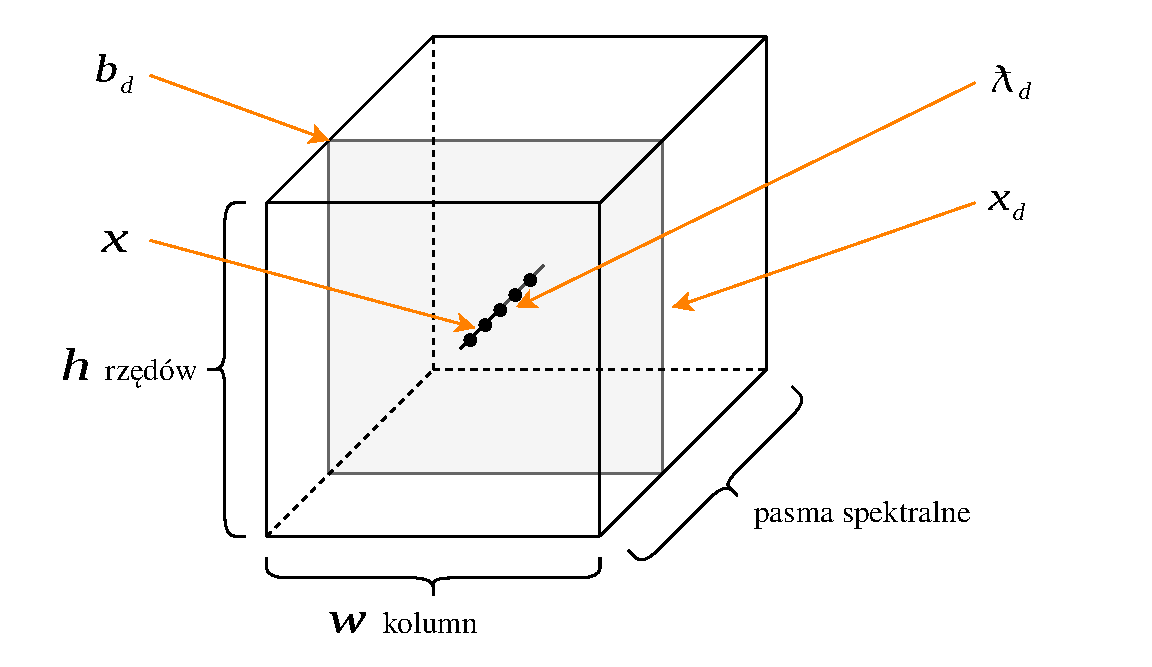
\includegraphics[width=0.75\linewidth]{rys02/multispectral-cube-vector}
	\caption{Schemat kostki wielospektralnego}
	\label{fig:multispectral-cube}	
\end{figure}

Na rysunku ~\ref{fig:multispectral-cube} zilustrowano układ danych w kostce wielospektralnej. Kostka taka składa się z~$n_x$ ($h$ rzędów na $w$ kolumn) pikseli $x$. Każdy piksel jest wektorem współczynników spektralnych o~długości  $n_D$, gdzie $n_D$ jest liczbą obrazów spektralnych, na które składa się dana wielospektralna. Każdy współczynnik $x_d$ jest wartością reakcji sensorycznej dla odpowiadającego pasma spektralnego $b_d$ skoncentrowanego wokół fali $\lambda_d$. W skrócie obraz wielospektralny jest zbiorem obrazów rejestrowanych przy użyciu fal elektromagnetycznych o~zadanych długościach. 


\subsection{Konsekwencje formatu danych}
Ze względu na swoją charakterystykę serie obrazów wielospektralnych mogą bezproblemowo osiągać rozmiary setek megabajtów, lub nawet gigabajtów. Zazwyczaj jednak obrazy są rejestrowane aparatem o~matrycy ok. 2 Mpix. Większość danych pochodnych, które są efektem analizy tego obrazu posiadają podobne rozmiary. Informacja ta jest kluczowa podczas projektowania mechanizmu zarządzania danymi w~takim systemie. Biorąc pod uwagę rozmiar danych mechanizm taki powinien:
\begin{itemize}
\item unikać tworzenia zbędnych kopi danych,
\item dokonywać obliczeń danych wyłącznie na żądanie,
\item zwalniać z~pamięci dane, które nie są już wykorzystywane przez aplikację.
\end{itemize}

\section{Dane w systemie Gerbil}

Oryginalny obraz wielospektralny jest traktowany jako dana wejściowa w systemie. Na jego podstawie powstają dane pochodne. Są to głównie kolejne obrazy oraz histogramy wielospektralne. Do stworzenia prototypu mechanizmu zarządzania danymi oraz procesem przetworzenia użyte zostały poniższe dane:
\begin{itemize}
	\item \index{image} \textbf{image} -- oryginalny obraz wielospektralny. Dana ta jest obliczana podczas inicjalizacji aplikacji. Użytkownik może wejść w interakcję z~systemem dopiero gdy image zostanie przetworzone.
	\item \index{ROI} \textbf{ROI (Region of Interest)} -- wyselekcjonowany podzbiór danych, w tym przypadku wybrane prostokątne zaznaczenie obrazu. Jest przechowywany jako współrzędne lewego górnego wierzchołka zaznaczenia, jego wysokość oraz szerokość,
	\item \index{image.IMG} \textbf{image.IMG} -- fragment obrazu oryginalnego zdeterminowany przez ROI,
	\item \index{image.NORM} \textbf{image.NORM} -- image.IMG po normalizacji wektorów składających się z~pikseli o~jednakowych współrzędnych na przestrzeni pasm spektralnych,
	\item \index{image.GRAD} \textbf{image.GRAD} -- gradient obrazu image.IMG,
	\item \index{image.PCA} \textbf{image.PCA} -- image.IMG po zastosowaniu metody PCA (analizy głównych składowych),
	\item \index{image.GRADPCA} \textbf{image.GRADPCA} -- image.GRAD po zastosowaniu metody PCA (ang. Principal Component Analysis - Analiza głównych składowych)\cite{PCA},
	\item \index{band} \textbf{bands.*.N} -- pojedynczy N-ty obraz spektralny danej reprezentacji image.* (przykładowo bands.NORM.6),
	\item \index{dist.IMG} \textbf{dist.IMG} - histogram wielospektralny obrazu image.IMG,
	\item \index{dist.tmp.IMG} \textbf{dist.tmp.IMG} - dana pomocnicza używana do uzyskania danej dist.IMG. 
\end{itemize}
Z racji, że jedne dane produkują inne, łatwo jest zdefiniować hierarchię danych w tym systemie.

\begin{figure}[ht]
	\centering
		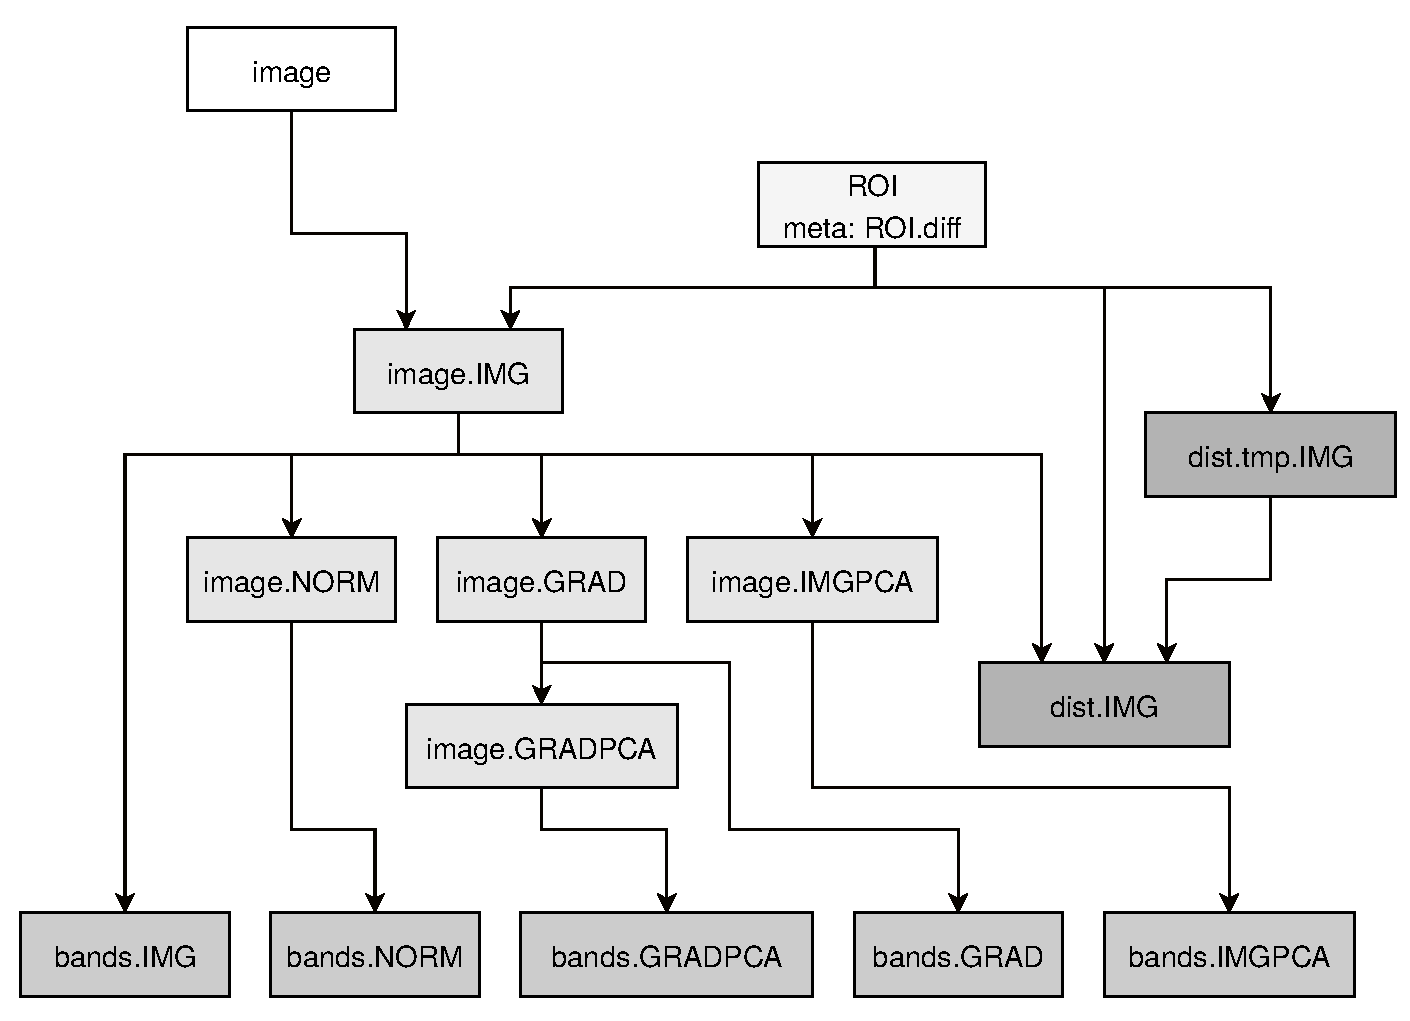
\includegraphics[width=0.7\linewidth]{rys02/data-dependencies}
	\caption{Graf zależności danych w systemie Gerbil}
	\label{fig:data-dependencies}	
\end{figure}

%\todo{Groty strzałek prawdopodobnie powinny być skierowane przeciwnie}
%\todo{Pojawiają się dziwne problemy z wstawieniem tego obrazka}

Na rysunku ~\ref{fig:data-dependencies} przedstawiono diagram zależności danych. Dane jednego koloru są do siebie semantycznie zbliżone. Przykładowo, image.NORM, image.GRAD, image.GRADPCA itp. są reprezentacjami obrazu oryginalnego. Dane posiadają również swoje metadane. Przykładowo metadaną ROI jest ROI.diff, które określa różnicę pomiędzy aktualnym a~poprzednim ROI. 

\subsection{Wpływ hierarchii danych na proces wykonania}
Analizując rysunek ~\ref{fig:data-dependencies} można dojść do wniosku, że proces przetworzenia danych jest dyktowany poprzez ich hierarchię. Przykładowo do obliczenia image.GRADPCA wymagane jest aby dane image, ROI, image.IMG oraz image.GRAD były już przetworzone. Dodatkowo można określić porządek, w którym te dane powinny zostać obliczone:

\begin{enumerate}[labelwidth=\widthof{\ref{last-item}},label=\arabic*.]
	\item image (podczas inicjalizacji systemu),
	\item ROI,
	\item image.IMG,
	\item image.GRAD,
	\item image.GRADPCA. \label{last-item}
\end{enumerate}

Scenariusz ten zakłada obliczenie każdej danej w hierarchii, co jest przypadkiem skrajnym. Często zdarza się, że pewna część danych jest aktualna. Wówczas przetwarzanie powinno rozpocząć się od pierwszej nieaktualnej danej znajdującej się najwyżej w hierarchii. 

Dodatkowo należy rozpatrzeć scenariusz równoległego wykonywania zadań. Zakładając, że aplikacja wyświetla jednocześnie dane image.NORM oraz image.GRAD, natomiast image.IMG zostało odświeżone, można dojść do wniosku, że system powinien w następnym kroku dokonać obliczeń obu danych (image.NORM i~image.GRAD). Obliczenia te można wykonać szeregowo bądź równolegle, wobec tego można zdefiniować opcjonalne wymaganie dla systemu zarządzania zadaniami jako możliwość równoległego przetwarzania zadań.

\chapter{Technologie wykorzystane w~systemie Gerbil}

Projekt jest rozwijany pod systemem operacyjnym Linux, dystrybucją Ubuntu 16.04.

\index{C++} \section{C++}
System Gerbil jest rozwijany w~języku C++. Jest to język programowania ogólnego przeznaczenia, ze szczególnym zastosowaniem w~tworzeniu systemów. C++ to język: 
\begin{itemize}
	\item wieloparadygmatowy -- pozwala na programowanie proceduralne, obiektowe, funkcyjne oraz ogólne,
	\item statycznie typowany -- zgodność typów jest sprawdzana w~trakcie kompilacji,
	\item pozwalający na bezpośrednie zarządzanie pamięcią,
	\item tworzony według zasady zerowego narzutu - elementy tego języka oraz proste abstrakcje muszą być optymalne (nie marnować bajtów pamięci ani cyklów procesora),
	\item umożliwiający tworzenie lekkich i~wydajnych abstrakcji \cite{Stroustrup}\cite{cplusplus}.
\end{itemize}

Język o~takiej charakterystyce jest dobrym wyborem do implementacji systemu analizy i~wizualizacji skomplikowanych danych.

W projekcie używany jest standard ISO/IEC 14882:2011 języka C++ oraz kompilator GCC w~wersji 5.4.0 \cite{C++11}.

\index{STL} \subsection{STL}
STL (ang. Standard Template Library) jest biblioteką standardową języka C++. Oferuje ona szereg kontenerów, klas, obiektów funkcyjnych oraz algorytmów. Składniki te opisane są w~standardzie ISO języka C++, oraz gwarantują identyczne zachowanie w~każdej implementacji \cite{Stroustrup}. Ułatwia to tworzenie aplikacji wieloplatformowych. Dzięki gotowym rozwiązaniom zawartym w~bibliotece standardowej, proces wytwarzania oprogramowania zyskuje na prostocie i~efektywności. 

\index{shared\_ptr} \subsubsection{\lstinline$shared_ptr$}
\lstinline$shared_ptr$ jest typem umożliwiającym reprezentację własności wspólnej. Wykorzystywany jest w~sytuacjach, gdy dwa (lub więcej) fragmenty kodu wymagają dostępu do danych, podczas gdy żaden nie jest odpowiedzialny za usunięcie tych danych. Obiekt \lstinline$shared_ptr$ jest rodzajem wskaźnika z~licznikiem wystąpień. Jeśli liczba obiektów wskazujących na konkretną daną spadnie do zera, dana ta jest usuwana \cite{Stroustrup}. 

\index{mutex} \subsubsection{\lstinline$mutex$}
Muteks jest obiektem typu \lstinline$mutex$, służącym do reprezentowania wyłącznych praw dostępu do konkretnego zasobu. Wykorzystuje się go do ochrony przed wyścigami do danych oraz synchronizacji dostępu do danych współdzielonych między wątkami.

Muteks może być w~posiadaniu tylko jednego wątku na raz. Zajęcie muteksu jest równoznaczne z~nabyciem wyłącznych praw własności do niego. Operacja zajmowania muteksu jest blokująca. Zwolnienie muteksu oznacza zrzeczenie się z~prawa własności do niego. Daje to możliwość zajęcia muteksu przez inne oczekujące wątki \cite{Stroustrup}.

%\subsubsection{\lstinline$condition_variable$}

\index{Qt} \section{Qt}

Qt jest platformą programistyczną wyposażoną w narzędzia pozwalające usprawnić proces wytwarzania oprogramowania oraz interfejsów użytkownika dla aplikacji desktopowych, wbudowanych bądź mobilnych \cite{Qtdoc}.

Platforma Qt posiada szerokie spektrum funkcjonalności. Między innymi są to:
\begin{itemize}
	\item system meta-obiektów,
	\item mechanizm sygnałów i~slotów służący do komunikacji pomiędzy obiektami,
	\item wbudowany system przynależności obiektów,
	\item wieloplatformowe wsparcie modułu wielowątkowości.
		
\end{itemize}

W systemie Gerbil jest wykorzystywane Qt w~wersji 5.7.

\index{sygnał} \index{slot} \subsection{Sygnały i~sloty}

Spośród rozszerzeń języka C++, jakie oferuje Qt, na szczególną uwagę zasługuje mechanizm sygnałów i~slotów. Dzięki niemu możliwe jest skomunikowanie dwóch dowolnych obiektów w~sposób alternatywny do użycia wywołań zwrotnych. 

Sygnał jest wysyłany, gdy nastąpi jakieś zdarzenie (np. naciśnięcie przycisku przez użytkownika), natomiast slot jest odpowiedzią na ten sygnał. Sygnatury sygnału i~slotu muszą być zgodne. Mechanizm ten jest luźno powiązany (ang. loosely coupled). Oznacza to, że klasa emitująca sygnał nie musi być świadoma klasy odbierającej. Sygnały i~sloty pozwalają na przekazanie dowolnej liczby argumentów dowolnego typu. Sygnały muszą zostać zadeklarowane po słowie kluczowym \lstinline$signals$. Z jednym slotem można połączyć dowolną ilość sygnałów, i~odwrotnie -- z~jednym sygnałem można skojarzyć dowolną ilość slotów.

Wszystkie klasy korzystające z~tego mechanizmu muszą w~swojej deklaracji zawierać makro \lstinline$Q_OBJECT$ oraz dziedziczyć (bezpośrednio bądź pośrednio) po klasie \lstinline$QObject$ \cite{Qtdoc}.


\subsubsection{Składnia} 
Sposób tworzenia połączeń zostanie zilustrowany na przykładzie. Za punkt wyjścia posłużą dwie klasy: \lstinline$Sender$ (Listing \ref{sender}) oraz \lstinline$Receiver$ (Listing \ref{receiver}).

\begin{minipage}{\textwidth}
	\begin{lstlisting}[label=sender,caption=Deklaracja klasy \lstinline$Sender$]
class Sender : public QObject
{
	Q_OBJECT
public:
	explicit Sender(QObject *parent = 0) : QObject(parent) {}
	
signals:
	void sendMessage(QString msg);
	
};
	\end{lstlisting}
\end{minipage}

\begin{minipage}{\textwidth}
	\begin{lstlisting}[label=receiver, caption=Deklaracja klasy \lstinline$Receiver$]
class Receiver : public QObject
{
	Q_OBJECT
public:
	explicit Receiver(QObject *parent = 0) : QObject(parent) {}
	
	void receiveMessageMethod(QString msg) {
		std::cout << "got message in method: " << msg;
	}
	
public slots:
	void receiveMessageSlot(QString msg) {
		std::cout << "got message: " << msg;
	}
};
	\end{lstlisting}
\end{minipage}

Z analizy listingów \ref{sender} oraz \ref{receiver} wynika, że klasa \lstinline{Sender} zawiera sygnał \lstinline{sendMessage}, natomiast klasa \lstinline{Receiver} zawiera publiczną metodę \lstinline{receiveMessageMethod} oraz publiczny slot \lstinline{receiveMessageSlot}.

W Qt występują dwa rodzaje składni pozwalające na ustanowienie połączenia. Jedna z~nich (starsza) pozwala na ustanowienie połączenia jedynie pomiędzy sygnałem a~sygnałem, bądź sygnałem a~slotem. Drugi rodzaj składni, wprowadzony w~Qt5, pozwala dodatkowo na nawiązanie połączenia pomiędzy sygnałem a~metodą klasy. Na listingu \ref{connectionsyntax} przedstawiony jest zarówno stary jak i~nowy zapis.

\begin{minipage}{\textwidth}
	\begin{lstlisting}[label=connectionsyntax, caption={Składnia tworzenia połączeń między obiektami},alsoletter={()[].=}]
Sender sender;
Receiver receiver;

//stara skladnia
//poprawne
QObject::connect(&sender, SIGNAL(sendMessage(QString)), &receiver, SLOT(receiveMessageSlot(QString)));
//niepoprawne
QObject::connect(&sender, SIGNAL(sendMessage(QString)), &receiver, SLOT(receiveMessageMethod(QString)));

//nowa skladnia
QObject::connect(&sender, &Sender::sendMessage, &receiver, &Receiver::receiveMessageMethod);
QObject::connect(&sender, &Sender::sendMessage, &receiver, &Receiver::receiveMessageSlot);
	\end{lstlisting}
\end{minipage}

Mechanizm sygnałów i~slotów jest powszechnie wykorzystywany w~systemie Gerbil do ustanowienia komunikacji pomiędzy obiektami. Używana jest zarówno stara jak i~nowa składnia.

\subsection{Wątek GUI oraz wątki robocze}
GUI (ang. Graphical User Interface) jest graficznym interfejsem użytkownika. Każda aplikacja jest uruchamiana w~osobnym wątku. Jest on nazywany wątkiem głównym (bądź "wątkiem GUI" w~aplikacjach Qt). Interfejs użytkownika rozwijany w~Qt musi zostać uruchomiony w~tym wątku. Wszystkie komponenty graficznego interfejsu użytkownika (ang. widget) oraz kilka klas pochodnych nie zadziałają w~wątkach pobocznych. Wątki poboczne są często nazywane "wątkami roboczymi", ponieważ wykorzystywane są aby odciążyć główny wątek od skomplikowanych obliczeń \cite{Qtdoc}. Gdyby te obliczenia były wykonywane w~ głównym wątku, aplikacja przestałaby być responsywna podczas obliczeń, co jest zawsze efektem niepożądanym.

\index{Boost} \section{Boost}
Boost jest kolekcją bibliotek do języka C++. Biblioteki te poszerzają funkcjonalności tego języka \cite{boost}. Wiele z~bibliotek rozwijanych przez Boost zostało włączonych do standardu C++. Z~perspektywy systemu Gerbil na specjalną uwagę zasługuje Boost.Any.



\subsection{Boost.Any}
W języku C++ kwestia przechowania obiektów dowolnego typu jest problematyczna, ponieważ jest to język statycznie typowany. 

\subsubsection{\lstinline$void*$}
W czystym C++ można użyć \lstinline$void*$. Do zmiennej typu \lstinline$void*$ można przypisać wskaźnik dowolnego typu poza wskaźnikiem do funkcji oraz wskaźnikiem do składowej. Aby użyć takiej zmiennej należy dokonać jawnej konwersji \lstinline$static_cast$. Do zastosowania \lstinline$void*$ w~kodzie wysokopoziomowym należy podchodzić z rezerwą. Może to wskazywać na błędy projektowe \cite{Stroustrup}.

\subsubsection{\lstinline$boost::any$}
Rozwiązaniem, które z~powodzeniem można stosować w~kodzie wysokopoziomowym jest właśnie klasa \lstinline$boost::any$. Jego zdecydowaną przewagą nad \lstinline$void*$ jest bezpieczny typowo interfejs. Jest to kontener opakowujący pojedynczy obiekt niemal dowolnego typu (obiekt musi posiadać możliwość inicjalizacji na bazie innego obiektu tego typu -- ang. copy-constructible).
Aby użyć obiektu przechowywanego przez \lstinline$boost::any$ należy dokonać rzutowania \lstinline$boost::any_cast$. Jeżeli zostanie podany typ, na który obiekt nie może zostać zrzutowany, zostanie zgłoszony wyjątek \lstinline$boost::bad_any_cast$ \cite{boost}.

\index{TBB} \section{Intel Threading Building Blocks}
Intel Threading Building Blocks (TBB) jest biblioteką szablonów ułatwiającą programowanie równoległe. W swojej ofercie posiada gotowe struktury danych oraz zrównoleglone algorytmy~\cite{tbb}.

W systemie Gerbil biblioteka TBB używana jest głownie do implementacji algorytmów przetwarzania obrazów wielospektralnych.

\index{OpenCV} \section{OpenCV}
OpenCV (Open Source Computer Vision Library) to biblioteka przeznaczona do rozpoznawania obrazów oraz uczenia maszynowego~\cite{opencv}.

Biblioteka ta znajduje wykorzystanie w~systemie Gerbil jako bogata baza struktur danych wykorzystywanych do przetwarzania obrazów oraz zaawansowanych algorytmów rozpoznawania obrazów.
\chapter{Aktualny stan projektu Gerbil}

\index{MVC} \section{Wzorzec MVC}

Aplikacja Gerbil jest zaprojektowana według wzorca MVC (Model-View-Controller) z~wykorzystaniem platformy Qt. MVC jest wzorcem architektonicznym używanym często do tworzenia interfejsów użytkownika. Podstawą MVC są trzy obiekty:
\begin{itemize}
	\item model -- komponent odpowiedzialny za serwowanie danych;
	\item widok -- komponent odpowiedzialny za wizualizację danych;
	\item kontroler -- komponent definiujący logikę, za pomocą której interfejs użytkownika odpowiada na jego żądania.
\end{itemize}
Podział tych ról można zaobserwować na rysunku ~\ref{fig:mvc}.

\begin{figure}[ht]
	\centering
	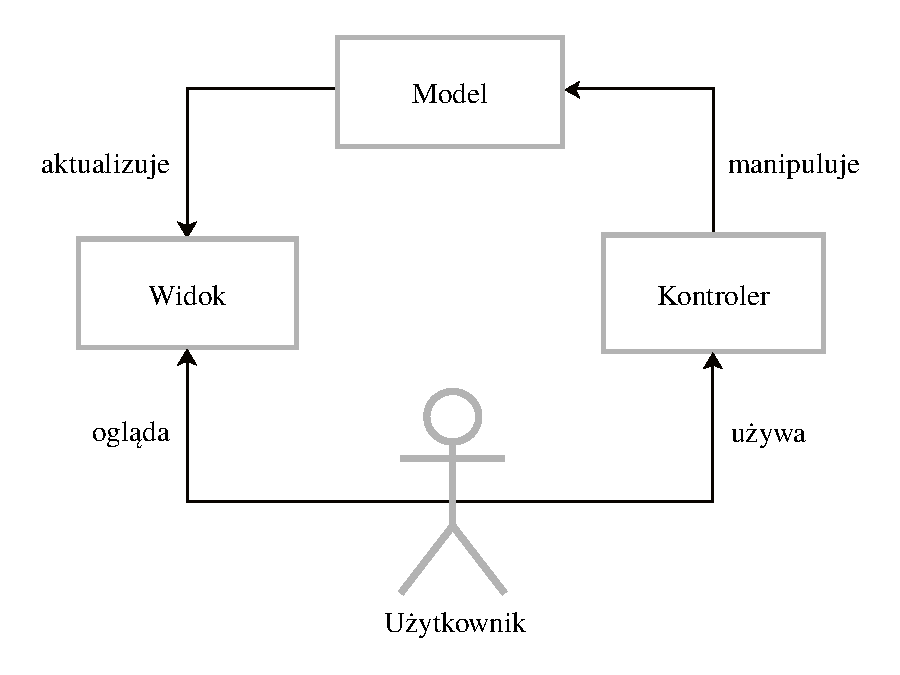
\includegraphics[width=0.7\linewidth]{rys04/mvc}
	\caption{Podział ról we wzorcu architektonicznym MVC}
	\label{fig:mvc}	
\end{figure}

Dzięki wykorzystaniu tego wzorca sposób przechowywania danych nie ma wpływu na to jak są one przedstawione użytkownikowi~\cite{Qtdoc}.

\section {Architektura aplikacji Gerbil}

W aplikacji Gerbil wzorzec MVC zastosowano w~sposób klasyczny: 
\begin{itemize}
	\item modele są odpowiedzialne za obliczenia danych oraz sygnalizowanie pojawienia się ich nowej wersji;
	\item widoki wyświetlają dane;
	\item kontrolery zajmują się kojarzeniem akcji użytkownika z~konkretną funkcjonalnością modelu.
\end{itemize}

Dodatkowo w~aplikacji występuje wątek roboczy. W nim uruchomiona jest kolejka zadań. Zadanie (obiekt klasy \lstinline$Task$) jest komponentem realizującym wykonanie czasochłonnego algorytmu analizy danych. Modele tworzą zadania i~przekazują je do kolejki. Kolejka przyjmuje zadania i~wykonuje je po kolei. W ten sposób skomplikowane obliczenia nie blokują wątku GUI, który pozostaje przez cały czas responsywny.

W takiej architekturze pojawia się problem dostępu do danych, ponieważ dwa wątki (wątek GUI, w~którym znajdują się komponenty MVC, oraz wątek roboczy, w~którym wykonywane są zadania) próbują uzyskać dostęp do tych samych danych. Zadania wykonywane w~tle powinny w~bezpieczny sposób dokonywać zapisu danych. Widoki zaś powinny być w~stanie bezawaryjnie wizualizować dane oraz dbać o~aktualność prezentowanych danych.

\subsection{Wady architektury}

System ten jest mocno zdecentralizowany. Na barkach kontrolerów spoczywa odpowiedzialność odpowiedniej propagacji sygnałów informujących o~nowej wersji danych, inwalidacji danych, jak również zapytań o~dokonanie nowych obliczeń. Prowadzi to do:
\begin{itemize}
	\item zaciemnienia kodu źródłowego zbędnymi instrukcjami warunkowymi,
	\item zignorowania pewnych sygnałów,
	\item podjęcia niewłaściwej decyzji.
\end{itemize}

Zarządzanie zadaniami również jest wadliwe. W przypadku gdy użytkownik poprzez interakcję z~systemem zleci wykonanie na raz kilku zadań dokonujących obliczeń na tych samych danych, system może zachować się w~sposób nieoczekiwany. Prowadzi to do zakończenia aplikacji z~powodu naruszenia ochrony pamięci. Nowa wersja systemu powinna w~najgorszym wypadku zakolejkować te zadania i~wykonać jedno po drugim.

Wiele komponentów interfejsu użytkownika przechowuje własne uchwyty do danych oraz ewentualnie muteks. Wobec tego same dokonują synchronizacji lub nie robią tego wcale. Nieprzemyślany model doprowadził do wielu patologii. Przykład stanowi używanie współdzielonych wskaźników do przekazywania danych, podczas gdy dane te z~założenia powinny być współdzielone.

\subsubsection{Konkluzja}

Aktualny model współdzielonych danych, w~powiązaniu z~modelem zarządzania nimi nie gwarantuje bezpiecznego dostępu do danych ani prawidłowego przebiegu procesu wykonania zadań. Biorąc pod uwagę wyżej wymienione problemy nowy mechanizm zarządzania danymi oraz procesem wykonania powinien: 
\begin{itemize}
	\item posiadać wewnętrzny mechanizm synchronizacji dostępu do danych,
	\item gwarantować bezpieczny dostęp do współdzielonych danych,
	\item gwarantować bezpieczne wykonanie zadań w~tle,
	\item gwarantować prawidłową kolejność procesu przetwarzania danych,
	\item posiadać scentralizowany mechanizm propagacji sygnałów,
	\item prawidłowo propagować informację o~dostępności nowej wersji danych,
	\item prawidłowo propagować informację o~żądaniu obliczeń nowych danych.
\end{itemize}






\chapter{Projekt nowego systemu}

\section{Zarys projektu}
Nowy system opiera się na komponencie zwanym Subscription Manager (SM). Jest on właścicielem wszystkich współdzielonych danych. Pozostałe komponenty uzyskują dostęp do danych przez obiekty nazywane Subscription (Subskrypcja). Prawa dostępu są przyznawane oraz kontrolowane przez SM. Dane tworzą graf zależności, który zapewnia automatyczne obliczanie potrzebnych danych. Komponenty typu Creator (odpowiedniki modeli we wzorcu MVC) kontrolują proces powstawania danej poprzez tworzenie odpowiednio sparametryzowanych zadań. Utworzone zadania trafiają do komponentu Task Scheduler, który zarządza ich wykonaniem.

\subsection{Przepływ danych w systemie} % TUTAJ ZDECYDOWAĆ SIĘ NA JEDNO ALBO DRUGIE (TO ALBO TO POWYŻEJ)


Obliczenia danych są wywoływane poprzez interakcję użytkownika z interfejsem graficznym. Dane są wizualizowane w konkretnych panelach. W celu prezentacji danych użytkownik musi aktywować dany panel. Z punktu widzenia systemu panel jest komponentem żądającym dostępu do danej w celu odczytu. W kodzie panela tworzony jest obiekt subskrypcji, który stanowi definicję takiego żądania. Obiekty tego typu stanowią interfejs pomiędzy komponentami żądającymi dostępu do danych a Subscription Managerem. Jeżeli dane są aktualne, panel otrzymuje stosowną informację. W ciele obsługi tej informacji dokonywany jest faktyczny dostęp do danych, dzięki czemu dana zostaje zaprezentowana w GUI. Możliwy jest również scenariusz, w którym żądana dana nie jest aktualna, bądź nie została jeszcze zainicjalizowana. Wówczas system wysyła informację do odpowiedniego komponentu typu Creator, który zadeklarował umiejętność wytworzenia tej danej. Komponent w odpowiedzi na informację tworzy obiekt Zadania oraz przekazuje go do Task Scheduler'a. Każdy obiekt zadania posiada pewne zależności wobec danych. Minimum stanowi żądanie dostępu do danej, która ma zostać obliczona, w celu zapisu. Zazwyczaj zależności dopełniają żądania dostępu do odczytu danych, od których obliczana dana zależy (o ile zależy). Task Scheduler tworzy odpowiednie obiekty subskrypcji dla danego zadania, na podstawie jego sygnatury zależnosci. Akcja ta może prowadzić do powstania kolejnych obiektów zadań (jeżeli zadanie żąda dostępu do danej, która również nie jest aktualna). Task Scheduler uruchamia powstałe zadania w osobnych wątkach. W momencie gdy dana zarządana przez użytkownika zostanie finalnie obliczona, panel GUI otrzymuje stosowną informację i może dokonać jej prezentacji.



\section{Model danych współdzielonych}
Ważne jest aby do roli danej współdzielonej można było promować każdą daną w systemie. Dlatego model danej współdzielonej nie może opierać się na interfejsie, który inne klasy by implementowały, lecz na opakowaniu, w które można każdą daną włożyć. Klasa danych współdzielonych nazwana została \lstinline$DataEntry$.


\subsection{Przechowywanie danych}
Kwestię przechowania dowolnego typu można rozwiązać poprzez wykorzystanie \lstinline$boost::any$. Natomiast problem uchwytu do danych, którego można użyć w różnych fragmentach kodu rozwiązuje \lstinline$std::shared_ptr$. Z tego powodu \lstinline$std::shared_ptr<boost::any>$ stanowi trzon modelu danych współdzielonych. Zarówno dane jak i towarzyszące im metadane są przechowywane w ten sposób. 
 
\begin{minipage}{\textwidth}
	\begin{lstlisting}[label=dataentry:alias, caption={Aliasy używane w kodzie aplikacji},alsoletter={()[].=}]
using handle = std::shared_ptr<boost::any>;
using handle_pair = std::tuple<handle, handle>;
	\end{lstlisting}
\end{minipage}

Aby kod był bardziej zwięzły stosowane są w nim aliasy (Listing \ref{dataentry:alias}). Pierwsza linia jest skróceniem zapisu typu uchwytu do danych, natomiast druga skraca zapis pary takich uchwytów (para uchwytów często jest wykorzysytywana do reprezentacji danych zagregowanych z metadanymi).

\subsection{Synchronizacja dostępu do danych}
Rozwiązanie to jednak nie likwiduje problemu synchronizacji dostępu do danych. Wobec tego model został wzbogacony o muteks oraz dwie zmienne warunkowe (Listing \ref{dataentry:sync}). Pierwsza zmienna warunkowa - \lstinline$not_reading$ służy do obsłużenia wątków oczekujących na dostęp do danych w celu zapisu, natomiast druga \lstinline$not_writing$ do obsługi wątków oczekujących na dostęp do danych w celu odczytu.

\begin{minipage}{\textwidth}
	\begin{lstlisting}[label=dataentry:sync, caption={Składowe klasy \lstinline$DataEntry$ zapewniające bezpieczne użycie w środowisku wielowątkowym},alsoletter={()[].=}]
std::mutex mu;
std::condition_variable not_reading;
std::condition_variable not_writing;
	\end{lstlisting}
\end{minipage}

Z pomocą tych narzędzi model udostępnia metody pozwalające na bezpieczny dostęp do danych w aplikacji wielowątkowej.

\begin{minipage}{\textwidth}
	\begin{lstlisting}[label=dataentry:sync:read, caption={Metody klasy \lstinline$DataEntry$ zapewniające bezpieczny odczyt danych współdzielonych w środowisku wielowątkowym},alsoletter={()[].=}]
handle_pair DataEntry::read()
{
	std::unique_lock<std::mutex> lock(mu);
	not_writing.wait(lock, [this]() {
		return !doWrite && initialized;
	});
	return handle_pair(data_handle, meta_handle);
}

void DataEntry::endRead()
{
	if (doReads == 0) not_reading.notify_one();
}
	\end{lstlisting}
\end{minipage}

Na listingu \ref{dataentry:sync:read} widoczna jest implementacja metod realizujących dostęp do danych w celu odczytu. 

W metodzie \lstinline$read$ tworzona jest blokada, która zajmuje mutex. Następnie wątek wywołujący metodę zostaje uśpione do momentu powiadomienia przez zmienną warunkową. Aby uniknąć fałszywych wybudzeń przekazywana jest dodatkowo lambda, która służy za predykat. Jeśli wartość zwrócona przez lambdę jest prawdziwa (zawarte jest w niej sprawdzenie czy wewnętrzny stan danej jest prawidłowy), wówczas wybudzenie jest słuszne. Po wybudzeniu zostaje zwrócona para uchwytów -- do danej oraz metadanej.

Metoda \lstinline$endRead$ służy do sygnalizacji zakończenia odczytu. W jej ciele wykonywane jest sprawdzenie czy wewnętrzny stan danej jest prawidłowy. Jeśli jest, wówczas zmienna warunkowa \lstinline$not_reading$ dokonuje przebudzenia jednego z wątków oczekujących na dostęp do danych w celu zapisu.

\begin{minipage}{\textwidth}
	\begin{lstlisting}[label=dataentry:sync:write, caption={Metody klasy \lstinline$DataEntry$ zapewniające bezpieczny zapis danych współdzielonych w środowisku wielowątkowym},alsoletter={()[].=}]
handle_pair DataEntry::write()
{
	std::unique_lock<std::mutex> lock(mu);
	not_reading.wait(lock, [this]() {
		return doReads == 0 && !doWrite;
	});

	return handle_pair(data_handle, meta_handle);
}

void DataEntry::endWrite()
{
	if (!doWrite) not_writing.notify_all();
}
	\end{lstlisting}
\end{minipage}

Analizując implementację metod pozwalających na bezpieczny zapis danych przedstawionych na listingu \ref{dataentry:sync:write} można dostrzec dużą analogie do metod z listingu \ref{dataentry:sync:read}. Jedyną zasadniczą różnicą jest fakt, że po zakończeniu zapisu zmienna warunkowa \lstinline$not_writing$ budzi wszystkie wątki oczekujące na dostęp w celu odczytu.

\section{Subscription oraz Subscription Manager}

Subscription Manager pełni rolę jednostki głównej w systemie. Jest on abstrakcją o poziom wyższą niż dane współdzielone. Komponent ten agreguje wszystkie takie dane oraz nimi zarządza. Do jego odpowiedzialności należą:
\begin{itemize}
	\item przyznawanie dostępu do danych,
	\item propagacja informacji o dostępności nowej wersji danych,
	\item propagacja informacji o żądaniu obliczeń nowych danych,
	\item zarządzanie cyklem życia danych,
	\item kontrola wewnętrznego stanu danych.
\end{itemize}

%Aby wyjaśnić funkcjonalności Subscription Managera, należy najpierw omówić przepływ danych w systemie. 



\section{Kreator (Creator)}

Kreator jest klasą semantycznie zbliżoną do Modelu z wzorca MVC. Zadaniem kreatora jest kontrola procesu wytworzenia danej. Interfejs zdefiniowany dla kreatora został przedstawiony na listingu \ref{creatorInterface}.

\begin{minipage}{\textwidth}
	\begin{lstlisting}[label=creatorInterface, caption={Interfejs klasy \lstinline$Creator$},alsoletter={()[].=}]
class Creator : public QObject
{
	Q_OBJECT
public:
	explicit Creator(SubscriptionManager& sm, TaskScheduler* scheduler,
						QObject *parent = 0);
	virtual ~Creator();

public slots:
	virtual void delegateTask(QString requestedId,
								QString parentId = "") = 0;
	void taskFinished(QString id, bool success);

protected:
	void registerData(QString dataId,
						std::vector<QString> dependencies);
	bool isTaskCurrent(QString id);

private:
	SubscriptionManager& sm;
	TaskScheduler* scheduler;
	
	std::map<QString, std::shared_ptr<Task>> tasks;

};
	\end{lstlisting}
\end{minipage}


Metoda \lstinline$registerData$ służy do rejestrowania danych. Za jej pomocą kreator zgłasza współdzielone dane, za które bierze odpowiedzialność. Każda dana współdzielona, aby istnieć w systemie, musi zostać zarejestrowana przez któryś z kreatorów. Do zarejestrowania danej wymagane jest jej ID oraz lista ID danych, od której owa dana jest zależna. Na listingu \ref{creator:registerData} został przedstawiony przykład rejestrowania współdzielonych. W pierwszych dwóch liniach zarejestrowane zostały dane, które są niezależne (lista ich zależności jest pusta). W trzeciej lini jest wyrażona rejestracja danej \lstinline$image.IMG$ oraz jej zależności od danych \lstinline$image$ oraz \lstinline$ROI$. Dzięki takiemu formatowi rejestrowania danych system jest w stanie stworzyć graf zależności danych, wykorzystywany do prawidłowej propagacji informacji.

\begin{minipage}{\textwidth}
	\begin{lstlisting}[label=creator:registerData, caption={Przykłady rejestrowania danych},alsoletter={()[].=}]
registerData("image", {});
registerData("ROI", {});
registerData("image.IMG", {"image", "ROI"});
	\end{lstlisting}
\end{minipage}

Z analizy listingu \ref{creatorInterface} wynika, że klasa implementująca interfejs Kreatora musi zdefiniować metodę \lstinline$delegateTask$ aby nie być klasą abstrakcyjną. Metoda ta jest kluczowa dla tego interfejsu, oraz bardzo ważna dla całego systemu. Ciało tej metody powinna stanowić obsługa żądania W definicji tej metody powinna znaleźć się obsługa żądania dokonania obliczeń danych. Żądanie takie może płynąć bezpośrednio od użytkownika, bądź w sposób pośredni, na skutek wewnętrznego mechanizmu systemu. Standardowym zachowaniem kreatora jest utworzenie odpowiedniego obiektu Zadania i przekazanie go do Task Scheduler'a. Teoretycznie możliwe jest, aby kreator sam dokonał obliczenia danej, zamiast tworzyć obiekt Zadania. Ta metoda jednak nie jest zalecana. Dopuszcza się jej stosowanie jedynie w przypadku nieskomplikowanych obliczeń na małych strukturach danych. 

Dodatkowo na uwagę zasługuje metoda \lstinline$isTaskCurrent$, dzięki której można sprawdzić, czy istnieje aktualnie zadanie o danym id, oczekujące na wykonanie, bądź aktualnie wykonywane. Informacja ta jest pomocna w tworzeniu rozbudowanej logiki kreatora.

\section{Zadanie (Task)}
Zadanie to komponent odpowiadający za bezpośrednie obliczenia danych. Służy zatem do zaktualizowania danej bądź jej inicjalizacji. Podstawową zasadą zadania jest to, że zawsze dokonuje on modyfikacji tylko jednej danej, natomiast może bazować na dowolnej liczbie danych, określanych jako "źródła". 


Każde zadanie posiada składową \lstinline$dependencies$, która jest listą jego zależności. Złożona jest ona z danej modyfikowanej oraz źródeł. Dla każdej danej w liście zależności określony jest również cel dostępu do niej (odczyt bądź zapis).

Id modyfikowanej danej musi zostać przekazane zadaniu jako parametr jego konstruktora. Identyfikatory źródeł również są przekazywane w konstrukorze, lecz w postaci mapy. W mapie tej kluczem jest identyfikator źródła, natomiast wartością identyfikator, według którego ta dana będzie rozróżniana wewnątrz zadania. Jest to zabieg zastosowany w celu ujednolicenia konwencji nazewniczej wewnątrz zadań. Zazwyczaj zadania posiadają jedynie jedno źródło, do którego odnoszą się za pomocą identyfikatora \lstinline$source$. Id danej modyfikowanej jest automatycznie mapowane na nazwę \lstinline$dest$. 

Zadanie, aby móc realizować dostęp do danych musi posiadać odpowiednie obiekty subskrypcji. Przeznaczona na nie jest składowa \lstinline$subscriptions$. Komponent nadrzędny, zarządzający zadaniem (Task Scheduler) jest zobowiązany do utworzenia dla niego właściwych obiektów subskrypcji (na podstawie jego zależności, zwracanych przez metodę \lstinline$getDependencies$) oraz przekazania ich poprzez metodę \lstinline$setSubscription$. Teoretycznie obiekt zadania może sam tworzyć subskrypcje, jednak nie jest to zalecane, a wręcz uznawane za błąd koncepcyjny. Przeznaczeniem zadania jest dokonywanie obliczeń na danych. Komponent tego typu nie powinien zajmować się zarządzaniem subskrypcjami.

Każde zadanie posiada własny identyfikator. Może być on przekazany jako parametr konstruktora. Jeżeli nie jest, wówczas identyfikatorem zadania staje się identyfikator modyfikowanej danej.

Zadanie posiada ściśle zdefiniowany interfejs, który został przedstawiony na listingu \ref{task:interface}.

\begin{minipage}{\textwidth}
	\begin{lstlisting}[label=task:interface, caption={Interfejs klasy \lstinline$Task$},alsoletter={()[].=}]
class Task : public QObject
{
	Q_OBJECT
public:
	explicit Task(QString target, std::map<QString, QString> sources);
	explicit Task(QString id, QString target, std::map<QString, QString> sources);

	virtual ~Task();
	virtual bool start() final;
	virtual void setSubscription(QString id, std::shared_ptr<Subscription> sub) final;

	std::vector<Dependency>& getDependencies();
	QString getId();

signals:
	void finished(QString id, bool success);

protected:
	virtual bool run() = 0;
	virtual std::shared_ptr<Subscription> sub(QString id) final;
	virtual bool subExists(QString id) final;
	virtual bool isCancelled();

private:
	QString id;
	std::vector<Dependency> dependencies;
	std::map<QString, QString> sources;
	std::map<QString, std::shared_ptr<Subscription>> subscriptions;

};
	\end{lstlisting}
\end{minipage}

Analizując listing \ref{task:interface} można ustalić, że jest to klasa abstrakcyjna. Klasy dziedziczące muszą zdefiniować metodę \lstinline$run$, aby nie być abstrakcyjne. Co więcej, wystarczające jest aby klasa zdefiniowała jedynie konstruktory oraz tą metodę, ponieważ właśnie ta ona przeznaczona jest do wykonywania obliczeń na danych. Wszelkie pozostałe metody mają charakter pomocniczy oraz są zapewnione przez klasę bazową. W ciele jej do obiektu subskrypcji można się odwołać za pomocą metody \lstinline$sub$. Można również sprawdzić czy dana subskrypcja została utworzona dzięki metodzie \lstinline$subExists$. Argumentem obu tych metod jest wewnętrzny identyfikator danej. Zadanie po zakończeniu metody \lstinline$run$ emituje sygnał \lstinline$finished$. Informacja taka może być przydatna dla kreatora zadania.

\section{Task Scheduler} 
Task Scheduler pełni zadanie komponentu zarządzającego zadaniami. Jak można wywnioskować z listingu \ref{scheduler:interface} klasa ta nie jest skomplikowana. Poprzez jedyną publiczną metodę \lstinline$pushTask$ trafiają do niego zadania stworzone przez kreatorów. Gdy zadanie zostanie przekazane do Task Scheduler'a, tworzy on subskrypcje dla niego. Funkcjonalność tą realizuje metoda \lstinline$createSubscriptions$. Zadanie, które posiada utworzone subskrypcje trafia do puli zadań (składowa \lstinline$taskPool$). Po dodaniu zadania do puli, pula zostaje przeiterowana w poszukiwaniu zadań gotowych do uruchomienia. Predykatem w tej sprawie jest Subscription Manager. Scheduler przekazuje mu listę zależności zadania a z powrotem otrzymuje wartość logiczną. Jeżeli jest ona równa \lstinline$true$, wówczas Task Scheduler uruchamia zadanie za pomocą metody \lstinline$startTask$. Jeżeli otrzymana wartość wynosi \lstinline$false$, Task Scheduler nie podejmuje żadnych akcji dla tego zadania i powraca do iteracji puli.

W metodzie \lstinline$startTask$ tworzony jest wątek, do którego przekazywany jest obiekt zadania. Wątek jest uruchamiany, a w nim uruchamiane zostaje zadanie. Dodatkowo ustanawiane jest połączenie, za pomocą którego po zakończeniu zadania Task Scheduler ponownie iteruje pulę zadań w celu znalezienia kandydata do uruchomienia. 

\begin{minipage}{\textwidth}
	\begin{lstlisting}[label=scheduler:interface, caption={Deklaracja klasy \lstinline$TaskScheduler$},alsoletter={()[].=}]
class TaskScheduler : public QObject
{
	Q_OBJECT
public:
	TaskScheduler(SubscriptionManager& sm);
	void pushTask(std::shared_ptr<Task> task);

private:
	void checkTaskPool();
	void startTask(std::shared_ptr<Task> task);
	void createSubscriptions(std::shared_ptr<Task> task);

	std::list<std::shared_ptr<Task>> taskPool;
	SubscriptionManager& sm;
};
	\end{lstlisting}
\end{minipage}
\chapter{Implementacja}

\section{Kompilacja projektu}
Kod źródłowy projektu można pobrać programem \lstinline$wget$ dostępnym w systemie GNU/Linux: \lstinline$wget https://github.com/ajaskier/gerbil/archive/distalpha.zip$. W~wyniku wykonania tej komendy pobrane zostanie archiwum o~nazwie \lstinline$gerbil-distalpha.zip$ zawierające kod źródłowy. Archiwum można rozpakować programem \lstinline$unzip$, który również jest dostępny w systemie \mbox{GNU/Linux:} \lstinline$unzip gerbil-distalpha.zip$. Po wykonaniu tej komendy kod źródłowy projektu znajdować się będzie w~katalogu \lstinline$gebril-distalpha$. Do zarządzania procesem kompilacji tego projektu wykorzystywane jest narzędzie \lstinline$CMake$~\cite{cmake}. Do rozwiązania zależności projektu można skorzystać z~interfejsu tego narzędzia o~nazwie \lstinline$ccmake$. W~programie \lstinline$ccmake$ należy wprowadzić ścieżki do wymaganych zależności projektu, zatwierdzić konfigurację klawiszem \lstinline$c$ po czym wygenerować szkielet projektu klawiszem \lstinline$g$. Po wykonaniu tego kroku można dokonać kompilacji projektu za pomocą programu \lstinline$make$.

\section{Integracja z~projektem Gerbil}
W skład pierwszej fazy integracji nowego systemu z~projektem Gerbil wchodzą 2 etapy:
\begin{enumerate}[labelwidth=\widthof{\ref{last-item2}},label=\arabic*.]
	\item zapewnienie funkcjonalności związanych z~reprezentacją obrazów,
	\item zapewnienie funkcjonalności związanych z~histogramami spektralnymi.
\end{enumerate}

W skład etapu pierwszego wchodzi: 
\begin{itemize}
		\item adaptacja istniejących klas zadań odpowiedzialnych za obliczenia konkretnych reprezentacji obrazów wielospektralnych do nowego interfejsu klasy \lstinline$Task$,
		\item adaptacja klasy \lstinline$ImageModel$ do nowego interfejsu klasy \lstinline$Model$,
		\item adaptacja widoków wyświetlających reprezentacje obrazów do nowego mechanizmu dostępu do danych współdzielonych.
\end{itemize}

Na drugi etap składa się:
\begin{itemize}
		\item zdefiniowanie procesu wykonania dla struktury reprezentującej histogram spektralny,
		\item adaptacja istniejących klas zadań odpowiedzialnych za obliczenie histogramu spektralnego,
		\item adaptacja klasy \lstinline$DistViewModel$ do nowego interfejsu klasy \lstinline$Model$,
		\item adaptacja widoków prezentujących histogramy spektralne do nowego mechanizmu dostępu do danych współdzielonych,	
\end{itemize}

Efektem tej fazy integracji powinna być aplikacja będąca podzbiorem funkcjonalności oryginalnej aplikacji Gerbil. Jej implementacja powinna być wystarczającym źródłem przykładów, aby zintegrować resztę komponentów projektu z~nowym systemem zarządzania danymi oraz procesem wykonania.

Etap pierwszy integracji został zakończony, aktualnie trwają prace nad ukończeniem etapu drugiego.





\bibliographystyle{plabbrv}

%UWAGA: bibliotekę referencji należy przygotować samemu. Dobrym do tego narzędziem jest JabRef.

%       Nazwę przygotowanej biblioteki wpisuje się poniżej bez rozszerzenia
%       (w tym przypadku jest to "dokumentacja.bib")

%\bibliography{dokumentacja}
%\appendix
%\include{dodatekA}
%\include{dodatekB}

\chapterstyle{noNumbered}
\phantomsection % sets an anchor
\addcontentsline{toc}{chapter}{Indeks rzeczowy}
\printindex

\begin{thebibliography}{9}
	
	\bibitem{PCA}
	\emph{Analiza głównych składowych}
  \url{https://pl.wikipedia.org/wiki/Analiza\_g\%C5\%82\%C3\%B3wnych_sk\%C5\%82adowych}
  (dostęp 23.11.2016).
	
	\bibitem{Stroustrup}
	Bjarne Stroustrup,
	\emph{Język C++. Kompendium wiedzy}.
	Wydawnictwo Helion, Gliwice,
	Wydanie IV,
	2014.
	
	\bibitem{cplusplus}
	\emph{Krótki opis języka C++}
	\url{http://www.cplusplus.com/info/description}
	(dostęp 31.10.2016).

	\bibitem{C++11}
	\emph{ISO/IEC 14882:2011}
	\url{http://www.iso.org/iso/catalogue_detail.htm?csnumber=50372}
	(dostęp 23.11.2016).
	
	\bibitem{Qtdoc}
	\emph{Dokumentacja Qt 5.7}
	\url{http://doc.qt.io/qt-5/index.html}
	(dostęp 30.10.2016).
	
	\bibitem{boost}
	\emph{Oficjalna strona Boost}
	\url{http://www.boost.org/}
	(dostęp 30.10.2016).
	
	\bibitem{tbb}
	\emph{Oficjalna strona Threading Building Blocks}
	\url{https://www.threadingbuildingblocks.org/}
	(dostęp 31.10.2016).
	
	\bibitem{opencv}
	\emph{Oficjalna strona OpenCV}
	\url{http://opencv.org/about.html}
	(dostęp 31.10.2016).
	
	\bibitem{cmake}
	\emph{Oficjalna strona CMake}
	\url{https://cmake.org/}
	(dostęp 06.12.2016).
	
\end{thebibliography}


\end{document}

